\documentclass[11pt]{article}

% ---------------------------------------------------------------------------
% Verifier Reach Is Spec Reach
% Experience / position paper for arXiv.
% All figures trace to committed, reproducible primaries (see CORRECTIONS.md data ledger).
% Build: pdflatex main && bibtex main && pdflatex main && pdflatex main  (or: tectonic -X compile main.tex)
% ---------------------------------------------------------------------------

\usepackage[utf8]{inputenc}
\usepackage[T1]{fontenc}
\usepackage{lmodern}
\usepackage{microtype}
\usepackage{amsmath,amssymb}
\usepackage{booktabs}
\usepackage{array}
\usepackage{xcolor}
\usepackage{graphicx}
\usepackage{tikz}
\usetikzlibrary{arrows.meta,positioning,shapes.geometric,calc}
\usepackage[margin=1in]{geometry}
\usepackage[hidelinks]{hyperref}
\usepackage{orcidlink}
\usepackage{enumitem}
\usepackage{caption}

\newcommand{\code}[1]{\texttt{#1}}

\title{\textbf{Verifier Reach Is Spec Reach:}\\[2pt]
       Moving Defect-Naming Forward in Agentic Coding Pipelines}
\author{David Sienkowski\,\orcidlink{0009-0007-5143-8925}\\\small research and measurements}
\date{Draft, 2026-06-26 --- experience/position paper}

\begin{document}
\maketitle

\begin{abstract}
Large-language-model verifiers are increasingly trusted to judge AI-generated code, yet they
systematically miss defects the specification never named---and do so confidently. On a corpus of
\emph{non-inferable} defects, where the correct behavior cannot be derived from the specification
plus general knowledge, a held-out test oracle caught $100\%$ ($3/3$ tasks) while a goal-backward
LLM verifier caught $0$ of $12$ verdicts, and was severely miscalibrated \emph{there}
(ECE $0.81$ on the clean non-inferable tasks versus $0.03$ on inferable tasks). The blind spot is
\emph{model-invariant}: it reproduces across three model tiers and across several independent
experiments, and a frontier model does no better than chance on it once a tie-break scoring artifact
is removed. A powered replication ($n=210$
verdicts, three model tiers, $5$ reps/cell, Wilson $95\%$ CIs) reproduces the blind spot at a
$100\%$ $[94\text{--}100]$ confident-false-pass rate and shows that resolving the surfaced edge into
the spec converts it to a $98\%$ $[91\text{--}100]$ catch; an independent,
CI-committed $43$-item eval built by the framework's maintainer corroborates this and refines it---the
fix is \emph{exogenous} tagging, not endogenous self-disconfirmation (which can even regress a correct
verdict). We argue the binding constraint
is \textbf{specification reach}, not verifier reasoning: a verifier can only catch what the spec
named. We present a productized response shipped into an open-source agentic coding framework
(GSD-Core): (1) a shape-classified \emph{edge-probe} that surfaces omitted edge cases at
specification time; (2) an adversarial \emph{prohibition-probe} that elicits must-NOT constraints
into a structured, verification-tiered contract; and (3) fail-closed verification that hard-gates
mechanically-checkable constraints and, for judgment-tier constraints it cannot confirm, abstains
(\code{insufficient\_spec}) rather than false-passes. We describe the unifying verification-tier
abstraction, deployment via maintainer-reviewed merges, and---honestly---the residual class where the
probe's recall gap leaves a held-out backstop irreplaceable. The contribution is a novel synthesis
plus original measurement, not a net-new concept; the headline blind-spot and fix are now powered with
confidence intervals on a self-validating harness, while the calibration and cross-construct corroboration
arms remain direction-finding on small samples.
\end{abstract}

% ===========================================================================
\section{Introduction}
% ===========================================================================

Agentic coding pipelines increasingly close the loop with an LLM \emph{verifier}: after a model
writes code, another model (or the same one in a fresh role) reads the code, the specification, and
the test artifacts, and renders a verdict---pass, or gaps found. The appeal is obvious. A verifier
needs no test harness, generalizes across languages, and reads intent the way a human reviewer does.
The risk is just as obvious in hindsight: a verifier that \emph{reasons} about correctness can be
confidently wrong, and unlike a failing test it offers no ground truth to contradict it.

This paper makes one claim and builds a system around it:

\begin{quote}
\textbf{A verifier's reach is the specification's reach.} An automated verifier can only catch a
defect whose correct behavior is recoverable from the spec plus general knowledge. When the spec
omits a domain edge, the verifier does not flag the omission---it fills the gap with a plausible
guess, marks the code passing at high confidence, and the bug ships unflagged.
\end{quote}

The lever this implies is counterintuitive. The instinct, when a verifier misses bugs, is to make
the \emph{judge} smarter: a stronger model, an ensemble, a debate, a calibrated confidence gate. We
show that on the defects that actually slip through, every one of those downstream moves is a no-op,
because the information the verifier needs was never in its input. The productive move is to widen
the input: move defect-naming \textbf{forward}, to specification time, so that the obligation the
verifier would have missed becomes something it can check.

\paragraph{Contributions.}
\begin{enumerate}[leftmargin=1.4em,itemsep=2pt]
\item \textbf{The measurement} (\S\ref{sec:measurement}): on a purpose-built non-inferable corpus, a
goal-backward verifier catches $0/12$ while a held-out oracle catches $100\%$, and is decisively
miscalibrated only in the non-inferable regime. The blind spot is model-invariant.
\item \textbf{The design principle} (\S\ref{sec:reach}): verifier reach $=$ spec reach. Convert
non-inferable obligations into inferable ones at spec time, rather than strengthening the judge.
\item \textbf{A shipped, tiered, fail-closed pipeline} (\S\ref{sec:system}): an edge-probe and an
adversarial prohibition-probe that write a verification-tiered \code{must\_haves} contract, plus a
verifier that abstains rather than false-passes on what it cannot confirm.
\item \textbf{Honest residual analysis} (\S\ref{sec:limitations}): the probe's recall is
classifier- and model-tier-dependent; a held-out backstop remains necessary for the residue.
\end{enumerate}

We frame these as \emph{confirmations and direction-finding plus a reproducible harness}, not as
discoveries. The samples are small (single- to double-digit per cell) and drawn from one framework;
the effects are large and one-sided, but they are leads, not proofs.

% ===========================================================================
\section{The Measurement}
\label{sec:measurement}
% ===========================================================================

\paragraph{Non-inferable corpus.} We built three self-validating tasks whose correct behavior cannot
be inferred from the spec we wrote plus general programming knowledge: half-to-even (banker's)
rounding, touching-interval merge ($[1,2]$ and $[2,3]$ merge or not?), and grapheme-aware string
truncation. A validation script proves each corpus is well-formed: the reference implementation
passes a held-out test that encodes the omitted edge, while the defective implementation passes the
visible spec-derived tests only. ``Non-inferable'' is relative to the spec given---a more complete
spec would make these inferable, which is precisely the point.

\paragraph{T1: held-out catches what the verifier cannot.}
Twelve inspection-only verifier subagents (opus and haiku, each emitting a verdict and a calibrated
confidence) reviewed the defective code. Table~\ref{tab:t1} states both denominators.

\begin{table}[h]
\centering
\caption{Catch rate of the non-inferable defect.}
\label{tab:t1}
\begin{tabular}{lc}
\toprule
\textbf{Mechanism} & \textbf{caught the omitted edge} \\
\midrule
Held-out test (encodes the omitted edge) & $3/3$ tasks $=\mathbf{100\%}$ (deterministic) \\
Goal-backward verifier (spec $+$ general knowledge) & $\mathbf{0/12}$ verdicts \\
\bottomrule
\end{tabular}
\end{table}

On the touching-interval task, all four verifiers passed the defective code, one explicitly reasoning
that strict \code{<} is ``defensible under a standard overlap definition''---a textbook non-inferable
miss: the spec never defined \emph{touching}, so there was no basis to flag it.

\paragraph{T2: the blind spot is a calibration failure, not a coverage gap.}
The same protocol scores the verifier's calibration across regimes (Table~\ref{tab:t2}). On inferable
defects the verifier is essentially perfect and well-calibrated. On the non-inferable clean tasks it
is right $13\%$ of the time while $93\%$ confident---an expected calibration error of $0.81$, and a
Brier score worse than chance. The verifier expresses $\approx\!0.93$ confidence whether it is right
(inferable) or wrong (non-inferable): \textbf{confidence is uninformative across regimes}. A
confidence gate cannot help, because the verifier is just as sure when it is blind.

\begin{table}[h]
\centering
\caption{Verifier calibration by regime (defective code; ground truth $=$ gap exists).}
\label{tab:t2}
\begin{tabular}{lccccc}
\toprule
\textbf{Regime} & $n$ & \textbf{accuracy} & \textbf{mean conf.} & \textbf{ECE} & \textbf{Brier} \\
\midrule
Inferable defects            & 16 & $100\%$ & $0.970$ & $\mathbf{0.030}$ & $0.001$ \\
Non-inferable (all tasks)    & 12 & $25\%$  & $0.927$ & $0.677$ & $0.644$ \\
Non-inferable (clean 02--03) & 8  & $\mathbf{13\%}$ & $0.930$ & $\mathbf{0.805}$ & $0.753$ \\
\bottomrule
\end{tabular}
\end{table}

\paragraph{The blind spot is model-invariant.}
The headline corpus is small, but the blind spot recurs across independent experiments, each attacking
the claim from a different angle:
\begin{itemize}[leftmargin=1.4em,itemsep=1pt]
\item A verifier-reach gauge (36 inspection verdicts across three tiers) finds true reach---verdict
\emph{and} correct identification of the planted edge---at $89\%$ on inferable defects but $0\%$ on
genuinely-arbitrary edges, unanimous across tiers.
\item A model-version probe finds uniform blindness across opus/sonnet/haiku (the omitted edge caught
$1/9$); verdicts barely drift, but confidence-while-wrong \emph{rises as model strength falls}
(opus $\approx\!0.65$ versus haiku $\approx\!0.96$).
\item An ordering-resolvability study finds non-inferable recovery at or barely above chance even at
the frontier ($14$--$29\%$ against a $16.7\%$ floor, the small excess a tie-break scoring artifact);
a $\sim\!30\times$ cost increase buys no additional recovery.
\item A repeatable-execution harness finds opus $\equiv$ haiku on an omitted rounding tie (capability
$75\%$, reliability $0\%$, byte-identical across reruns).
\end{itemize}
Re-running a bigger model never closes the gap; only spec reach does.

\paragraph{A powered replication (n=210).}
We replicate the blind spot at scale on a purpose-built corpus (four self-validated non-inferable tasks
$+$ one inferable control, $\times$ three tiers $\times$ five reps; $n=210$ verdicts; \code{analyze.mjs}
recomputes every figure deterministically from the recorded \code{verdicts.tsv}, reporting Wilson $95\%$
confidence intervals). The harness now \emph{self-validates} non-inferability locally: \code{validate.mjs}
confirms, for every non-inferable task, that the defective implementation passes the visible
spec-derived tests yet fails a held-out edge test (the inferable control is exempt by design), so the
non-inferable property is proven in-repo rather than only by reference. Each task is run under three spec
states (Table~\ref{tab:t4}). \emph{Narrow} (the omitted edge stripped, no abstain option) reproduces the
$n=12$ blind spot, powered: confident-false-pass $=\mathbf{100\%}$ $[94\text{--}100]$, uniform across
tiers ($n=20$ each). \emph{Surfaced-resolved} (the omitted edge written into the spec as an explicit
criterion) converts blind-spot into catch $=\mathbf{98\%}$ $[91\text{--}100]$, residual false-pass $2\%$
$[0\text{--}9]$---mechanizing verifier-reach $=$ spec-reach. \emph{Surfaced-unresolved} (the \emph{real}
compiled edge-probe tag appended, abstention available) drives $40\%$ $[29\text{--}53]$ honest abstention,
tier-gated: opus $65\%$ $[43\text{--}82]$ honest (abstain$+$catch) $>$ sonnet $55\%$ $[34\text{--}74]$ $>$
haiku $0\%$ $[0\text{--}16]$ (flag-deaf). The inferable control shows $100\%$ catch with $0\%$
$[0\text{--}20]$ over-abstention---the real tagger, unlike a deliberately-false oracle, did not induce
needless deferral. The run was adversarially audited at the transcript level: no hallucination, exact
model pinning ($15$ per tier), an independent re-parser reproducing all $210$ verdicts, $0/45$
cross-condition reads under per-condition isolated build directories, and $0$ code executions.

\begin{table}[h]
\centering
\caption{Powered edge-probe-residual replication (canonical \code{v4}; $n=210$ verdicts: four
non-inferable tasks $\times$ three tiers $\times$ five reps; Wilson $95\%$ CIs from \code{analyze.mjs}).
The blind spot (narrow false-pass) and the fix (surfaced-resolved catch) are both near-saturated;
surfacing the edge without resolving it converts false-passes into honest abstentions.}
\label{tab:t4}
\begin{tabular}{lcccc}
\toprule
\textbf{Condition (non-inferable tasks)} & $n$ & \textbf{false-pass} & \textbf{abstain} & \textbf{catch} \\
\midrule
Narrow (omitted edge stripped)            & 60 & $\mathbf{100\%}$ [94--100] & $0\%$ [0--6]    & $0\%$ [0--6] \\
Surfaced-unresolved (real edge-probe tag) & 60 & $57\%$ [44--68]            & $40\%$ [29--53] & $3\%$ [1--11] \\
Surfaced-resolved (edge written to spec)  & 60 & $2\%$ [0--9]               & $0\%$ [0--6]    & $\mathbf{98\%}$ [91--100] \\
\bottomrule
\end{tabular}
\end{table}

\paragraph{The recall gap: an edge-probe miss is necessary but not sufficient.}
Does the residual false-pass concentrate on the tasks the edge-probe's recall \emph{misses}? We widened
the non-inferable set to seven tasks ($n=300$, identical protocol, adding two MISS-classified
categories---null-vs-absent and idempotency/text-wrap) and re-estimated the gap. At the aggregate level
there is \emph{no} clean separation: in surfaced-unresolved, edge-probe-HIT tasks false-pass at $73\%$
$[59\text{--}84]$ and MISS tasks at $56\%$ $[41\text{--}69]$, CIs overlapping---and MISS is
counterintuitively the \emph{lower} of the two. The per-task breakdown supplies the real finding.
Idempotency---a complete miss, since the probe never fires for text-shape functions---is a genuine blind
spot: $93\%$ $[70\text{--}99]$ false-pass surfaced-unresolved, $100\%$ in narrow. Precision/tie (a miss
under the tagger version that scored it) is likewise a blind spot ($67\%$ $[42\text{--}85]$). But
null-vs-absent, though an edge-probe miss, is \emph{caught} ($7\%$ $[1\text{--}30]$ false-pass; $0\%$ in
narrow), because the null-property-preservation rule is already derivable from the spec's existing ``for
each key not present in target'' language. The mechanism is therefore conditional: \textbf{an edge-probe
miss is necessary but not sufficient for a verifier blind spot---the omitted edge must also be
non-derivable from the spec's remaining obligations.} Two caveats bound the claim. The MISS categories
were \emph{hand-selected} for edge-probe blindness, so this is a conditional/existence statement, not an
unbiased population miss-rate; and the precision/tie miss label is tagger-version-dependent---the
currently-deployed tagger would re-classify it as a hit, leaving two MISS categories. The held-out
backstop stays irreplaceable precisely on the genuine blind spots within this set.

\paragraph{Abstention is configuration-dependent.}
Two further arms---identical model, fixtures, and ground truth, varying only the verifier's I/O and
prompt wording---show that the \emph{absolute} abstention rate is a property of the setup, not the model.
Reading the spec and code from files and replying in TSV roughly doubles abstention versus receiving them
inline ($20\%$ $[12\text{--}32]\to40\%$ $[29\text{--}53]$, surfaced-unresolved); a forceful ``you MUST
abstain'' instruction lifts it to $91\%$ $[83\text{--}95]$, dragging even flag-deaf haiku from $0\%$ to
$80\%$. The blind spot and the fix are robust across every arm; the abstention rate is not. This
reinforces the program guardrail: \textbf{abstention is not a primary mechanism}---its rate can be dialed
by the harness, so the irreducible residual still needs a held-out backstop.

\paragraph{Independent corroboration.}
The replication above lived in a personal fork the framework's CI could not reach, so the maintainer
independently rebuilt and committed an in-CI behavioral eval
(\code{tests/verdict-eval/}): a $43$-item corpus---vetted item-by-item by an independent model for
blind-safety, realism, correct ground truth, and correct class (inferable $12$, domain-knowledge $10$,
spec-silent $14$, clean $7$)---recorded blind on two models (Sonnet, Haiku) across three modes,
$258$ judgments, $0$ malformed, $65$ CI tests green. Recordings are committed transcripts replayed by
a deterministic token-regex judge, so the result is key-free and reproducible. Two harnesses---ours and
the maintainer's, blind to each other, different models and prompts---land the same conclusion
(Table~\ref{tab:t5}).

This run also sharpens the construct: ``non-inferable'' is not one thing. It splits into a
\emph{domain-knowledge} class (a boundary a capable self-check can surface from its own training, e.g.
banker's rounding) and a \emph{truly spec-silent} class (genuinely ambiguous without the spec). The
blind spot proper is the spec-silent class, and only exogenous tagging closes it: spec-silent catch
rises from $36\%$ (Sonnet) / $43\%$ (Haiku) at baseline to $79\%$ / $71\%$ under exogenous tags, and
the confident-false-pass rate drops from $64\%$ / $57\%$ to $21\%$ / $29\%$. Endogenous
\emph{self-disconfirmation} (re-derive criteria, then rebut your own verdict) is inert-to-harmful on
the capable tier: net zero on Sonnet, where it \emph{regressed} a correct flag
(\code{pagination-index-base}, FLAG$\to$PASS---the self-check talked itself out of a real catch); on
Haiku it gives a modest $+7$--$10$pp. A distinct endogenous \emph{abstention} mode (``don't pass unless
confident''; a fourth \#1637 arm, not in Table~\ref{tab:t5}) is a cheap routing win---spec-silent catch
$36\%\!\to\!57\%$ (Sonnet) and $43\%\!\to\!64\%$ (Haiku), $+21$pp on both, at zero over-abstention
cost---but it routes rather than resolves: it is the verify-time trigger for exogenous resolution, not
a substitute for it.

\begin{table}[h]
\centering
\caption{Powered, CI-committed eval (maintainer-built; $43$ items, $2$ models, $258$ blind judgments).
Recall $=$ defect-catch rate per class; CFP $=$ confident-false-pass on the spec-silent class.
figures from open-gsd/gsd-core\#1637 (\code{tests/verdict-eval/}).}
\label{tab:t5}
\begin{tabular}{llccccc}
\toprule
model & mode & inferable & domain-know. & spec-silent & spec-silent CFP & clean prec. \\
\midrule
Sonnet & baseline             & $100\%$ & $80\%$  & $36\%$          & $64\%$          & $100\%$ \\
Sonnet & endogenous (disconf.)& $100\%$ & $80\%$  & $36\%$          & $64\%$          & $100\%$ \\
Sonnet & exogenous (tag)      & $100\%$ & $100\%$ & $\mathbf{79\%}$ & $\mathbf{21\%}$ & $100\%$ \\
Haiku  & baseline             & $100\%$ & $60\%$  & $43\%$          & $57\%$          & $86\%$  \\
Haiku  & endogenous (disconf.)& $100\%$ & $70\%$  & $50\%$          & $50\%$          & $86\%$  \\
Haiku  & exogenous (tag)      & $100\%$ & $100\%$ & $\mathbf{71\%}$ & $\mathbf{29\%}$ & $100\%$ \\
\bottomrule
\end{tabular}
\end{table}

\paragraph{Hygiene.} Two contamination corrections were applied mid-experiment and recorded: a
function-name leak and a false-positive confound on the rounding task (segregated), plus comment
stripping of ground-truth hints. A separate cross-version run showed that leaving answer hints in the
corpus inflated the apparent catch rate roughly $3\times$ (from $3/9$ to $1/9$ once sanitized)---a
reminder that the honest number is the lower one.

% ===========================================================================
\section{Verifier Reach Is Spec Reach}
\label{sec:reach}
% ===========================================================================

Why is a non-inferable defect \emph{unverifiable} rather than merely hard? Because the verifier has
nothing to check against. Goal-backward verification compares the implementation to the
specification's stated obligations plus general convention. When the obligation was never stated and
no convention determines it, the comparison is vacuous: any behavior is ``consistent with the spec.''
The verifier is not failing to reason; it is reasoning correctly over an input that does not contain
the answer. This is why a held-out test and a strong goal-backward verifier ``draw from the same
source---the spec'': across the corpus, held-out tests add no marginal catch \emph{on inferable
defects}, and their only demonstrated marginal value is exactly on the non-inferable residue.

The implication inverts the usual remedy. Rather than strengthen the reader, surface the missing
obligation into the spec. We observe the converse directly: when a weak overseer is handed structured
\code{must\_haves} that name the spec-defined correctness condition, it matches a strong reviewer on
spec-defined defects---the artifact, not the model, supplies the reach. So the highest-value
investment is spec completeness, with a held-out test as the backstop for edges the author knows but
cannot fully articulate.

\paragraph{The general law.} The non-inferable blind spot is the special case of a pipeline-wide
pattern: \emph{each stage's reach equals its input artifact's reach}. A planner cannot integrate a
seam the plan never pinned (in a controlled run, independent executor waves integrated $0/9$ on an
unpinned interface versus $9/9$ when the plan pinned it); a verifier cannot catch what the spec
omitted; a gray-area resolver cannot resolve what the criteria never named. The failure mode at every
stage is what the artifact silently got wrong or left out---never what it left visibly blank---and
the fix is always to widen or reconcile the artifact upstream, never to deploy a stronger reader
downstream.

\paragraph{Connections to engineering folklore.} Two well-worn observations sharpen the framing.
Goodhart's law---when a measure becomes a target, it ceases to be a good measure---predicts the
failure precisely: the moment an agent loop optimizes for ``the verifier returns pass,'' the verdict
stops tracking correctness, and it stops first exactly where the verifier is blind. Our defenses are
the standard Goodhart defenses---pair the proxy (the verdict) with an outcome measure that is harder
to fake (a held-out test), and audit the proxy-to-reality relationship (the exogenous non-inferable
tag). Linus's law---``given enough eyeballs, all bugs are shallow''---fails for this bug class for the
same reason it usually succeeds: it relies on cognitive diversity, but a non-inferable edge is an
\emph{assumption every reviewer shares}, because the missing information is absent from the artifact
rather than hidden in the code. More model-eyeballs (an ensemble, a debate) cannot make shallow a bug
that is invisible to all of them; the review that helped in practice (\S\ref{sec:deployment}) was a
human bringing outside knowledge the artifact lacked.

% ===========================================================================
\section{System}
\label{sec:system}
% ===========================================================================

The pipeline (Figure~\ref{fig:pipeline}) has two spec-time instruments that write a single
verification-tiered contract, and one verify-time disposition that fails closed.

\begin{figure}[h]
\centering
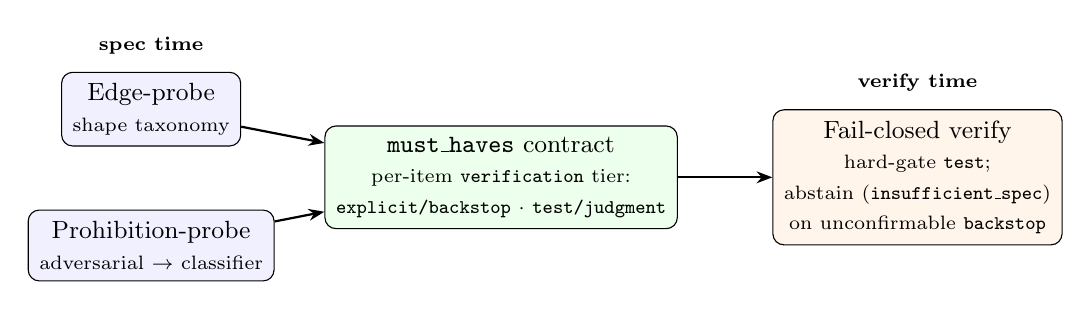
\begin{tikzpicture}[
  node distance=8mm and 12mm,
  box/.style={draw,rounded corners,align=center,inner sep=4pt,minimum height=9mm,font=\small},
  probe/.style={box,fill=blue!6},
  contract/.style={box,fill=green!7},
  verify/.style={box,fill=orange!8},
  arr/.style={-{Stealth[length=2mm]},thick}
]
\node[probe] (edge) {Edge-probe\\\scriptsize shape taxonomy};
\node[probe,below=of edge] (proh) {Prohibition-probe\\\scriptsize adversarial $\to$ classifier};
\node[contract,right=22mm of $(edge)!0.5!(proh)$] (mh)
  {\code{must\_haves} contract\\\scriptsize per-item \texttt{verification} tier:\\\scriptsize
   \texttt{explicit/backstop} $\cdot$ \texttt{test/judgment}};
\node[verify,right=of mh] (ver) {Fail-closed verify\\\scriptsize hard-gate \texttt{test};\\\scriptsize
   abstain (\texttt{insufficient\_spec})\\\scriptsize on unconfirmable \texttt{backstop}};
\draw[arr] (edge) -- (mh);
\draw[arr] (proh) -- (mh);
\draw[arr] (mh) -- (ver);
\node[font=\scriptsize,above=1mm of edge] {\textbf{spec time}};
\node[font=\scriptsize,above=1mm of ver] {\textbf{verify time}};
\end{tikzpicture}
\caption{Pipeline: two spec-time probes write a verification-tiered \code{must\_haves} contract;
the verifier hard-gates mechanically-checkable items and abstains on what it cannot confirm.}
\label{fig:pipeline}
\end{figure}

\subsection{Edge-probe: shape-classified completeness}
At spec time, the edge-probe classifies each requirement by \emph{shape} (numeric-range, collection,
text, stateful, I/O) and, from a fixed eight-category checklist (boundaries, adjacency/touching,
empty/degenerate inputs, encoding, ordering/stability, precision/overflow, idempotency,
concurrency), raises the edges that the requirement's shape implies. Each raised edge gets a
disposition: \emph{specify} (becomes an acceptance criterion), \emph{backstop} (a held-out test
stands in; the edge is tagged non-inferable), \emph{dismiss} (with a recorded reason), or
\emph{defer} (an explicit planner assumption). The category taxonomy is sound; the binding weakness
is the prose$\to$shape classifier (\S\ref{sec:limitations}). The instrument is most distinct from
sampling-based clarification (\S\ref{sec:related}) in that it emits a \emph{persistent, verifiable
contract} rather than a one-shot question.

\subsection{Prohibition-probe: adversarial must-NOT elicitation}
Shape classification surfaces what a requirement should \emph{handle}; it is silent on what a feature
must \emph{not become}. A second instrument elicits prohibitions in two stages. Stage~1 (recall) asks
adversarially, per requirement: \emph{``what could this feature silently become that the author would
not want, but the spec does not forbid?''}---over-generating candidates. Stage~2 (precision) runs a
one-pass classifier that keeps only the genuine values/safety prohibitions and drops routine
engineering must-nots. Measured: the adversarial framing reaches $25/25$ holistic prohibitions and
$17/17$ canon-less (product-values) prohibitions \emph{including} haiku at $6/6$, where a
role-played ``three amigos'' review reaches only $9/17$ on canon-less cases; the classifier collapses
a $\sim\!9.3$-item list to $\sim\!2.3$ while retaining the ground-truth prohibition $8/8$ and
promoting $0/8$ pure-engineering items to prohibitions on a clean battery. Confirmed prohibitions
become \code{must\_haves.prohibitions} entries.

Crucially, the difficulty of prohibitions is \emph{not} a negation problem. When the same violating
code is shown to verifiers under positive (``must'') versus negative (``must NOT'') framings, catch
rate is identical ($9/9 = 9/9$, gap $0.00$, $\approx\!0.99$ confidence). The real difficulty is
\textbf{scope}: a prohibition quantifies universally over the repository, while a per-phase inspector
samples. The remedy is therefore a repository-wide deterministic check, not a more negation-aware
reader.

\subsection{Fail-closed verification and abstention}
Every contract item carries an orthogonal \texttt{verification} tier. \emph{Test-tier} items
(mechanically checkable by a negative test, lint, or AST rule) \textbf{hard-gate} the verify phase
and fail closed if the check cannot be run. \emph{Judgment-tier} items (irreducible values rules)
and \emph{backstop}-tagged truths route, when unconfirmable, to a distinct verdict
\code{insufficient\_spec} $\to$ \code{human\_needed}---the verifier abstains rather than emitting a
confident green. The disposition ships in the probe core as the truth-axis counterpart to the
verified prohibition disposition \code{dispositionForProhibition()} (\code{probe-core.cts}).

The decisive finding is that abstention must be \textbf{exogenous}. Table~\ref{tab:t3} shows the
confident-false-pass rate on the blind spot by condition: a tag that \emph{forces} deferral drops it
from $100\%$ to $17\%$, while an ``abstain if you are unsure'' instruction (endogenous) reaches only
$67\%$ and fires only on the \emph{salient} ambiguity it happens to notice---never on the true blind
spot, which the model cannot feel. Two costs bound the win: a \emph{false} non-inferable tag makes a
strong model over-abstain on a real spec-determined bug ($33\%$ over-abstention), so detector
precision is load-bearing; and the weakest tier (haiku) is flag-deaf, heeding the tag inconsistently.
Abstention is therefore exogenous \emph{and} tier-pinned to a capable model. It also does not
\emph{recalibrate}: ECE among the verdicts that stay decisive on non-inferable tasks nudges from
$0.93$ to $0.98$. The deliverable is fewer decisions in the blind spot, not better-calibrated ones.
These are direction-finding numbers ($n=27$). At scale the powered replication
(\S\ref{sec:measurement}, $n=210$) shows the same shape with a \emph{real} edge-probe tag:
surfaced-unresolved drives $40\%$ honest abstention, tier-gated (opus $65\%$ honest, haiku $0\%$), and
surfaced-\emph{resolved} reaches $98\%$ catch; the independent CI-committed eval (Table~\ref{tab:t5})
corroborates---exogenous tagging lifts spec-silent catch to $71$--$79\%$ and roughly thirds the
confident-false-pass rate---and sharpens one caveat: endogenous \emph{self-disconfirmation} (as opposed
to abstention) is not merely weak but can be \emph{harmful}, regressing a correct flag on the capable
model. Abstention routes the case to exogenous resolution; it does not diagnose, and self-disconfirmation
should not ship as a verification control.

\begin{table}[h]
\centering
\caption{Confident false-pass on the non-inferable blind spot, by abstention condition
($n=27$, 1 rep).}
\label{tab:t3}
\begin{tabular}{lcccc}
\toprule
\textbf{Condition} & $n$ & \textbf{false-pass} & \textbf{abstain (honest)} & \textbf{mean conf. of false-pass} \\
\midrule
Baseline (no abstain option)        & 6 & $\mathbf{100\%}$ & $0\%$  & $0.93$ \\
Endogenous (self-judged abstain)    & 6 & $67\%$ & $33\%$ & $0.96$ \\
Exogenous (tagged non-inferable)    & 6 & $\mathbf{17\%}$ & $\mathbf{83\%}$ & $0.98$ \\
\bottomrule
\end{tabular}
\end{table}

A useful property of exogenous abstention: it routes correctly \emph{even with the wrong diagnosis}.
Under tagging, verifiers abstained on the grapheme task while citing unrelated reasons (a negative
\code{max}, a null coercion)---they identified the wrong gap and still took the right action. A
mechanism that produces correct \emph{deferral} without correct \emph{identification} is exactly what
a blind spot needs, because if the verifier could name the true edge it would not be blind.

\subsection{The unifying primitive}
Edges and prohibitions look like different features, but they share one structure: each contract item
carries a \texttt{verification} tier, and \emph{abstention is the disposition when that tier cannot be
discharged}. Mechanically checkable obligations hard-gate; unconfirmable ones abstain. This collapses
``surface the gap,'' ``write the must-NOT,'' and ``don't fake the green'' into a single contract with
a single fail-closed rule.

% ===========================================================================
\section{Deployment}
\label{sec:deployment}
% ===========================================================================

The pipeline ships in the open-source GSD-Core framework. As of this draft the merged pieces are:
the edge-probe (issue \#550 / PR \#584); recall sharpening (\#1108) and unclassified-edge surfacing
(\#1117); the prohibition-probe (\#644 / PR \#1149); test-tier enforcement, the fail-closed hard-gate
(\#1273); the deterministic check-descriptor that lets the verifier locate a check rather than invent
one (\#1301); and the honest verifier / truth-axis abstention (\#1154 / PR \#1738). A
machine-proven fail-first guard (\#1314) is in flight.

We treat the maintainer review itself as an external validation signal. Across many rounds, an
independent maintainer hit both failure modes the program had predicted before adopting the fix: spec
prose-drift, and a self-graded review that rationalized away its own findings (observed as malicious
compliance on a separate PR). The test-tier enforcement that now hard-gates mechanically-checkable
prohibitions was seeded directly by a maintainer's observation that the prohibition-probe's safety
half shipped before its enforcement half. This is one ecosystem and one maintainer---weak evidence in
isolation---but it is adversarial, independent, and it moved the design.

The validation went further than review. Because our headline abstention numbers lived in a personal
fork and were not reproducible from the framework's repository, the maintainer independently built the
powered, CI-committed eval of \S\ref{sec:measurement} (Table~\ref{tab:t5}) to re-test the claim from
scratch---a separate corpus, separate models, blind to ours. It corroborated the load-bearing result
(exogenous tagging closes the spec-silent gap), refined the construct (the domain-knowledge vs
spec-silent split), and \emph{overturned} an encouraging first-run signal (endogenous
self-disconfirmation, $0\%\!\to\!67\%$ at $n=3$, collapsed to inert-or-harmful when powered). An
independent party re-deriving, sharpening, and partially falsifying a claim is the strongest external
signal in this paper.

% ===========================================================================
\section{Related Work}
\label{sec:related}
% ===========================================================================

\paragraph{Spec completeness and clarification.}
ClarifyGPT~\cite{clarifygpt} detects ambiguity by sampling code completions and asking clarifying
questions where they disagree. The non-inferable blind spot is precisely where samples \emph{agree}
on the wrong behavior, so consistency-sampling is silent there; the edge-probe is shape-driven and
emits a persistent, verifiable contract rather than a one-shot question. Boundary Value
Analysis~\cite{myers2011art} is a decades-old test-design technique; our placement of it
\emph{upstream, at spec-authoring time, as a completeness gate wired into the verifier} is the
repositioning, not the technique.

\paragraph{Negative and prohibition constraints.}
Omission-constraint decay~\cite{omissiondecay} shows prohibitions are fragile under context
(adherence $73\%\rightarrow33\%$ by turn~16 over thousands of trials), motivating a persistent
contract over an in-prompt instruction. Enforcement frameworks such as Safety
Chip~\cite{safetychip} compile constraints into checkable form. Our distinction is spec-time
elicitation paired with tiered, fail-closed verification.

\paragraph{Abstention and selective prediction.}
Conformal Abstention~\cite{conformalabstention} offers hallucination-rate guarantees via conformal
prediction. AbstentionBench~\cite{abstentionbench} benchmarks abstention on \emph{underspecified}
inputs and finds it unsolved, with ``scaling models of little use''---which independently corroborates
our model-invariant blind spot. Our distinction is a coding-agent verify-phase abstention gated by an
\emph{exogenous} inferability tag (not self-judged confidence) and emitted as a first-class
\code{insufficient\_spec} verdict.

\paragraph{LLM-as-judge weakness.}
Studies of verification for code generation report that homogeneous or limited test suites let subtle
faults go undetected and recommend held-out tests~\cite{rethinkingverification}; surveys catalog
LLM-as-judge weaknesses~\cite{llmjudgesurvey}. These corroborate verifier overconfidence; the
spec-reach framing---and the specific claim that overconfidence \emph{concentrates} on non-inferable
requirements---is ours.

% ===========================================================================
\section{Limitations}
\label{sec:limitations}
% ===========================================================================

\begin{itemize}[leftmargin=1.4em,itemsep=2pt]
\item \textbf{Sample sizes; still not a large study.} Our calibration result is $n=12$; the powered
replication is $n=210$ ($5$ reps/cell, CIs reported) with a $n=300$ extension over seven non-inferable
tasks for the recall-gap, but the MISS categories underlying that finding were hand-selected for
edge-probe blindness---a conditional/existence claim, not an unbiased population miss-rate---and one
MISS label is tagger-version-dependent; the independent corroboration is $n\approx10$--$14$ per
class, two models, one run/seed. The spec-silent class has no ground-truth ``right answer'' without the
spec, so even exogenous tagging cannot reach $100\%$ there, and the inferable/non-inferable label is
itself model-dependent. Effects are large and monotone, but we report leads plus reproducible harnesses,
not a powered multi-seed study, and there is no preregistration.
\item \textbf{Recall residual.} The shape-classification step
is a leaky abstraction: on prose alone the deterministic classifier under-fires
($\sim\!48\%$ of applicable edges missed on one corpus, worse on a terser second corpus), because
terse prose yields no shape and therefore no edge. An
LLM-in-the-loop classifier recovers most of this on a sonnet-class model or better (under-fire
$\sim\!14\%$ at sonnet, near-zero at opus), but the weakest tier is high-variance and unreliable. On the
genuine blind spots---edges the probe fails to \emph{name} \emph{and} that the spec's other obligations
do not imply---the verifier still false-passes at $67$--$93\%$ even when the edge is surfaced unresolved;
so the pipeline is not a complete fix, and a held-out backstop remains necessary
for the residue.
\item \textbf{Abstention is not free.} A false non-inferable tag induces over-abstention on real
spec-determined bugs; the weakest tier is flag-deaf. Abstention quality is bounded by detector
precision and model tier.
\item \textbf{Single ecosystem.} All deployment evidence is from one framework and one maintainer.
Any cross-model or cross-family verifier recommendation is \emph{unvalidated}---every verifier
subagent in these experiments was from a single model family.
\item \textbf{Model-version sensitivity.} Abstention is tier-gated and confidence-while-wrong varies
by tier; results may shift across model generations.
\end{itemize}

% ===========================================================================
\section{Conclusion}
% ===========================================================================

The overconfident verifier is not a reasoning failure to be out-reasoned; it is a reach failure to be
out-specified. A verifier catches what the spec named, so the productive intervention is to name more,
earlier---shape-classified edges and adversarially-elicited prohibitions written into a
verification-tiered contract---and to make verification fail honestly, abstaining on what it cannot
confirm rather than stamping a confident green. We have shipped this into an open-source framework and
measured where it works and where it does not. The honest bottom line is a synthesis with an original
measurement and a residual that still needs a held-out backstop---move defect-naming forward, make
verification fail closed, and keep the oracle for the edges no spec yet reaches.

\paragraph{Reproducibility.} The paper, the reproducible experiments behind every headline number, and
the design docs are collected in a public artifact repository:
\url{https://github.com/davesienkowski/verifier-reach-is-spec-reach}. The
$n=210$ powered replication and its $n=300$ recall-gap extension ship their recorded \code{verdicts}
TSVs, the \code{analyze.mjs} scorer that recomputes every figure with Wilson $95\%$ CIs (no model
calls), and a \code{validate.mjs} gate that locally proves each task's non-inferability. The independent corroboration is a committed, key-free,
CI-green artifact in the framework repository (\code{tests/verdict-eval/}, open-gsd/gsd-core\#1637):
committed transcripts replayed by a deterministic judge, per-slice metrics locked as a golden
fixture---anyone can re-run it. Every figure in this paper traces to a committed primary that
recomputes deterministically; the smallest, single-rep results would still benefit from additional reps
and confidence intervals, a camera-ready refinement rather than an open question of support.

\section*{Acknowledgements}
The research thesis and measurements are the author's own work. The pipeline features ship in the
open-source GSD-Core project and are community contributions; merges and review were performed by the
project's maintainers, whose adversarial review materially improved the design.

\bibliographystyle{plain}
\bibliography{refs}

\end{document}
